\documentclass{article}
\usepackage[utf8]{inputenc}
\usepackage{graphicx}
\usepackage{hyperref}

\newtheorem{theorem}{Theorem}[section]
\newtheorem{lemma}{Lemma}[section]

\begin{document}

\title{Byzantine Agreement with Unknown Participants and Failures report}
\author{Denes Laszlo Fekete}
\maketitle   

\section{Introduction}
This report summarizes the Byzantine Agreement with Unknown Participants and Failures paper by Pankaj Khanchandani and Roger Wattenhofer, the program created for the paper  and the experiments belonging to the program. The figures and terminologies are taken from this paper\cite{khanchandani2021byzantine}. The repository is available on github\footnote{\url{https://github.com/denes710/bft_cup_inf_lab}}.

The task of participants in a distributed system is to agree on a shared opinion. To achieve this, an instance of a Byzantine agreement problem must be solved. In this paper, the researchers provide an approach in which participants do not need to be aware of the total number of participants in the system (\(n\)) and an upper bound on the number of Byzantine participants (\(f\)). This is a unique approach to the problem, in contrast to most existing solutions in which participants are required to be aware of these mentioned numbers. In this approach the system is synchronous. The paper contains a proof that shows that synchrony is necessary as an agreement with probabilistic termination is impossible in a semi-synchronous or asynchronous system if participants are not aware of the mentioned numbers. Synchronous or asynchronous system if the participants are unaware of \(n\) and \(f\). Authors give Byzantine agreement algorithms for reliable broadcast, approximate agreement, rotor-coordinator, early terminating consensus and total ordering in static and dynamic systems, all with the optimal resiliency of \(n > 3f\).

\section{Byzantine Agreement with Unknown Participants and Failures}
\subsection{Model}
The description of the model is as follows in the paper, and the most important parts of the model definition will be discussed further on. The system consists of n nodes, out of which at most f are faulty nodes. The faulty nodes can behave in any way whatsoever, also known as Byzantine behavior.We call the non-Byzantine nodes correct. The nodes have unique identifiers, which are not necessarily consecutive. As it has been mentioned before the system is synchronous and the computation proceeds in rounds. In each round, every node receives the messages that were sent to it in the previous round. The identifier of a node is included in the message. The receiver of the message can decipher its sender. Thus, a Byzantine node cannot forge its identifier when communicating directly. Byzantine nodes can send duplicate messages across rounds but duplicate messages from the same node in a round are simply discarded. The following algorithms are used in the id-only model and will be discussed briefly in this report: reliable broadcast, rotor-coordinator, consensus, parallel version of the consensus and an algorithm for achieving approximate agreement and total ordering of events in a dynamic network using the mentioned parallel version of the consensus.

\subsection{Reliable Broadcast}
The authors used reliable broadcast\cite{srikanth1987simulating} abstraction to provide message consistency in correct nodes. The main part of the algorithm is that all correct nodes know the same messages. Thus Byzantine nodes cannot send contradictory messages to correct nodes,  however they can send false information, which is solved by each correct node having consistent false information. The pseudo code of the algorithm is shown in Figure~\ref{reliable_fig}.

\begin{figure}[hbt!]
    \centering
    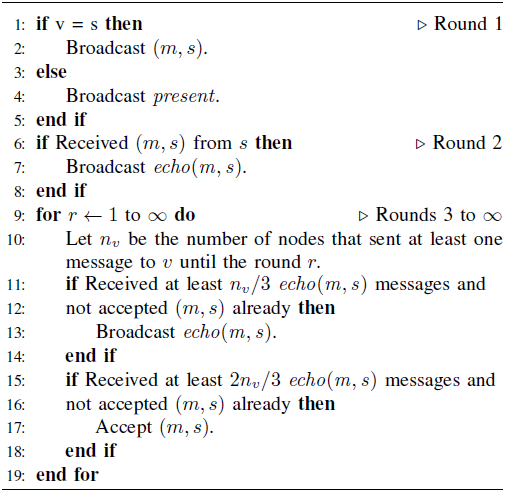
\includegraphics[width=0.70\textwidth]{figures/reliable_broadcast.png}
    \caption{Reliable broadcast pseudocode.\label{reliable_fig}}
\end{figure}

The formalised version of reliable broadcast in the paper is the following. Let s be a designated node that may or may not be correct and (m, s) be a message broadcast by s. The message (m, s) is reliably broadcast when the following three properties are satisfied.

\begin{itemize}
  \item Correctness: If s is correct, then each correct node accepts (m, s).
  \item Unforgeability: If a correct node accepts a message (m, s) and s is a correct node, then the message (m, s) was broadcast or sent to all the nodes by the node s.
  \item Relay: If a correct node accepts the message (m, s) in a round r, then each correct node accepts the message (m, s) by the round r + 1.
\end{itemize}

The belonging lemmas and theorem to this algorithm in the paper, which satisfy all the properties of the reliable broadcast and will be used in other algorithms later, are the following:
\begin{lemma}
If \(n > 3f\), then the given algorithm satisfies the correctness property of the reliable broadcast.
\end{lemma}
\begin{lemma}
If \(n > 3f\) and a correct node v receives at least \(n_v/3\) copies of a message m from distinct nodes in a round r, then at least one of those messages was sent by a correct node.
\end{lemma}
\begin{lemma}
If \(n > 3f\), then the given satisfies the unforgeability property of the reliable broadcast.
\end{lemma}
\begin{lemma}
If \(n > 3f\) and a correct node v receives at least \(2n_v/3\) copies of a message m in a round r, then every correct node u receives at least \(n_u/3\) copies of m in the round r.
\end{lemma}
\begin{lemma}
If \(n > 3f\) then the given satisfies the relay property of the reliable broadcast.
\end{lemma}
\begin{theorem}
If \(n > 3f\), then algorithm in Figure~\ref{reliable_fig} satisfies the properties of the reliable broadcast in the id-only model.
\end{theorem}
\subsection{Rotor-coordinator}
Every node selects a coordinator for every round. The purpose of Rotor-Coordinator is to ensure that these selected coordinators are the same in correct nodes. The algorithm builds on there being a correct coordinator proceeding \(f + 1\) rounds, after \(f + 1\) coordinators are selected, because there are only \(f\) faulty nodes. If a correct node terminates in a round, then all other correct nodes terminate in the same round as well. 

\begin{figure}[hbt!]
    \centering
    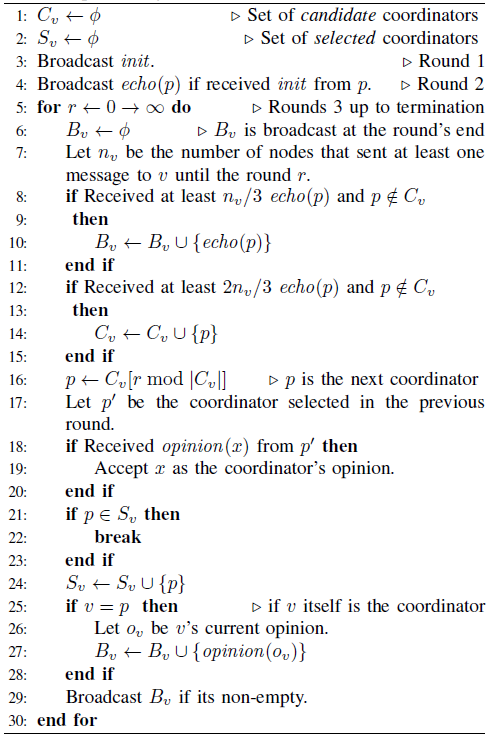
\includegraphics[width=0.70\textwidth]{figures/rotor_coordinator.png}
    \caption{Rotor-coordinator pseudocode.\label{rotor_coordinator_fig}}
\end{figure}

The terminology of the Rotor-coordinator in the paper is the following. We call a round a good round if the same node p was selected as a coordinator by every correct node and the node \(p\) is correct. We will call a round as a silent round if the set \(C_v\) remains unchanged for every correct node \(v\). A non-silent round is a round that is not silent.

The belonging lemmas and theorem to this algorithm in the paper, which will be used in other algorithms later, are the following:
\begin{lemma}
If a correct node \(v\) adds \(p\) to the set \(C_v\) in a round r, then any correct node \(u \neq v\) adds p to the set \(C_u\) by the round \(r + 1\).
\end{lemma}
\begin{lemma}
If \(n > 3f\), then every correct node witnesses at least one good round until it terminates.
\end{lemma}
\begin{theorem}
If \(n > 3f\), then every correct node terminates in \(O(n)\) rounds and there is a round in which every correct node accepts the opinion of a common and a correct coordinator node.
\end{theorem}

\subsection{Consensus}
\begin{figure}[hbt!]
    \centering
    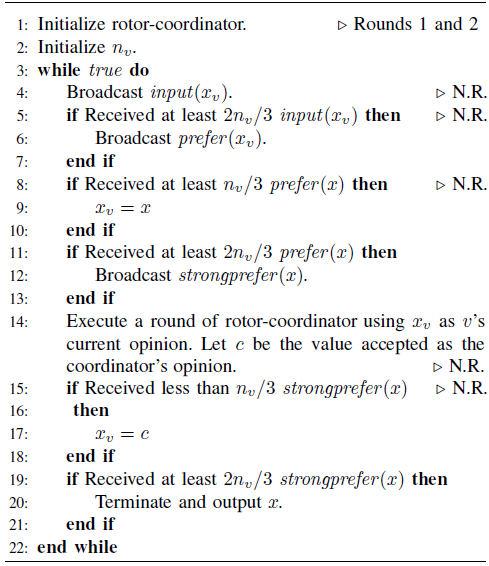
\includegraphics[width=0.70\textwidth]{figures/consensus.png}
    \caption{Consensus pseudocode.\label{consensus_fig}}
\end{figure}
The authors gave an \(O(f)\) round consensus algorithm. The algorithm in Figure~\ref{consensus_fig} gives an algorithm based on \cite{berman1992optimal}. A phase is an iteration of the loop. A node only accepts a message if the sender nodes send their identifiers during initialization. Otherwise, a node discards this message. During initialization, the sent messages with identifiers are counted to define the number of nodes in the consensus.

The belonging lemmas and theorem to this algorithm in the paper, which will be used in other algorithms later, are the following:
\begin{lemma}
If \(x_v = x\) for every correct node at the start of the phase, all the nodes terminate with the output \(x\) at the end of the phase.
\end{lemma}
\begin{lemma}
If a correct node u receives \(2n_u/3\) copies of a message \(m\) and a correct node \(v\) receives \(2n_v/3\) copies of a message \(m'\) in the same round, then at least one correct node sent both \(m\) and \(m'\) in the previous round.
\end{lemma}
\begin{lemma}
If a correct node terminates in a phase, then all other correct nodes have the same opinion at the end of the phase.
\end{lemma}
\begin{lemma}
If the coordinator is correct and none of the correct nodes have terminated, then all the correct nodes have the same opinion by the end of the phase.
\end{lemma}
\begin{theorem}
Algorithm in Figure~\ref{consensus_fig} solves consensus in \(O(f)\) rounds in the id-only model.
\end{theorem}

\subsection{Parallel version of consensus}
Using the previously discussed consensus algorithm, the authors defined a parallel version of consensus where each correct node can submit multiple opinions.

\begin{figure}[hbt!]
    \centering
    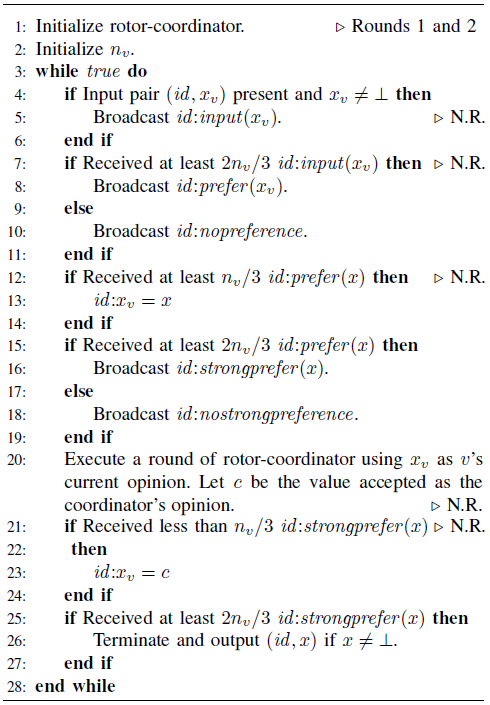
\includegraphics[width=0.70\textwidth]{figures/parallel_consensus.png}
    \caption{Parallel version of consensus pseudocode.\label{parallel_consensus_fig}}
\end{figure}

The formalised version of the parallel version of consensus in the paper is the following. Every correct node \(v\) has a set of \(k_v\) input pairs. 
The \(EarlyConsensus(id)\) algorithm is described in Figure~\ref{parallel_consensus_fig}, where every correct node \(v\) has at most one input pair \((id, x_v)\). The parallel consensus properties are the followings:
\begin{itemize}
  \item Validity: If (id, x) is an input pair of every correct node and \(x \neq \perp\), then all the correct nodes must output the pair (id, x).
  \item Agreement: If a correct node v outputs a pair \((id_v, x_v)\), then all other correct nodes must output \((id_v, x_v)\) as well.
  \item Termination: Every correct node outputs a set of pairs in finite number of rounds.
\end{itemize}

\subsection{Application to dynamic networks}
To solve the problem of total ordering of events in a dynamic system, authors used the current round number as consensus identifier. This identifier is included in the corresponding messages. The later discussed output chain is ordered by this identifier. Thus, multiple parallel consensus instances can run at the same time. A node has to broadcast its willingness to all other nodes to take part in the network and has to indicate if leaving the network.

The formalised version of the maximum number of rounds in the paper is the following. Consider a round \(r'\) that is final with respect to \(v\). Since each phase of \(EarlyConsensus(id)\) is five rounds and the initialization is two rounds, the parallel consensus instance \(r'\) terminates by \(r' +5f'_r +2\) rounds, where \(f'_r\) is the number of faulty nodes in the round \(r'\).

The formalised version of the sequence output in the paper is the following. The nodes agree on the sequences that they output. Let \(T^r_v\) be the sequence output by a correct node v at the end of round \(r\). The algorithm in Figure~\ref{dynamic_network_fig} satisfies the following two agreement properties:
\begin{itemize}
  \item Chain-prefix: For any pair of correct nodes \(u, v\), either \(T^r_u\) is a prefix of \(T^r_v\) or \(T^r_v\) is a prefix of \(T^r_u\).
  \item Chain-growth: For every correct node \(v\), events are appended to \(T^r_v\) over time, if a correct node submits an event in every round.
\end{itemize}

\begin{figure}[hbt!]
    \centering
    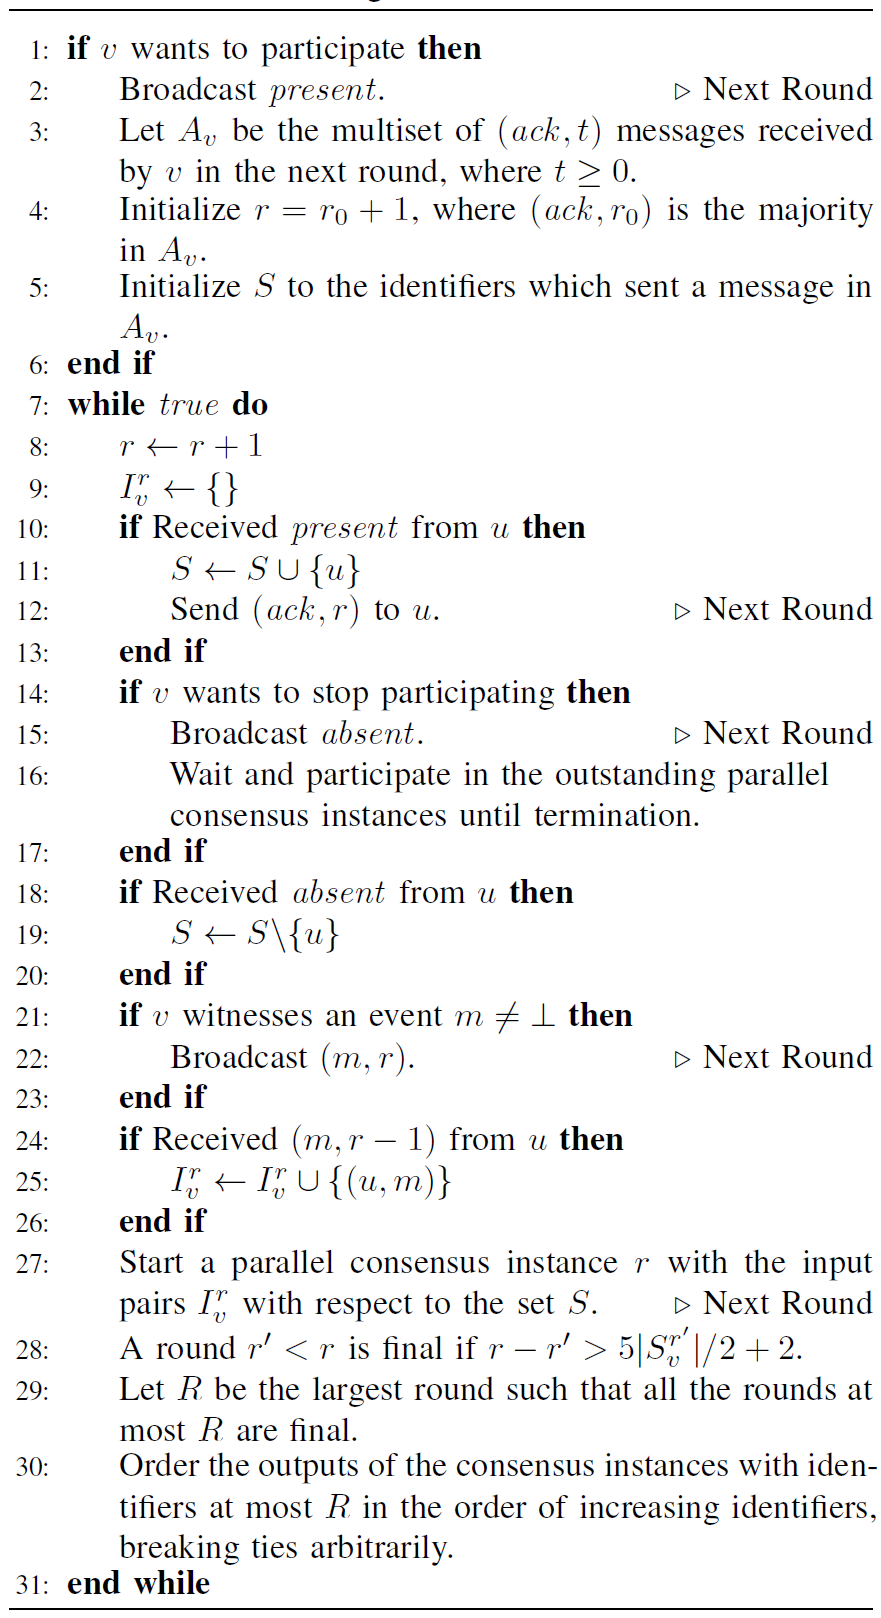
\includegraphics[width=0.70\textwidth]{figures/dynamic_network.png}
    \caption{Application to dynamic network pseudocode.\label{dynamic_network_fig}}
\end{figure}

\newpage
\section{The program}
The program is written in Python3. It consists of two parts, backend(backend/main.py) and frontend(frontend/main.py). The backend simulates the given scenario from the input file and if necessary then creates an output file as an input file for the frontend.
The input and output files are json files. The frontend can show all information about a given consensus from this input file. The program is using the following libraries:

\begin{itemize}
  \item argparse
  \item datetime
  \item logging
  \item json
  \item PyQt5
\end{itemize}

The backend part of the program has a simple command-line interface with the following parameters:

\begin{itemize}
  \item input-file
  \item no-logging
\end{itemize}

\begin{figure}[hbt!]
    \centering
    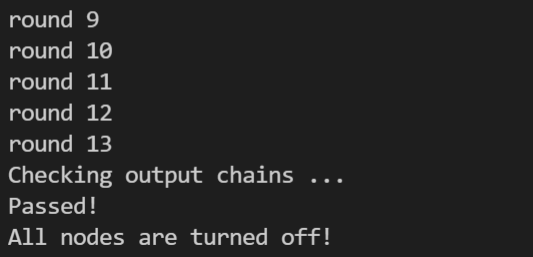
\includegraphics[width=0.70\textwidth]{figures/terminal_output.png}
    \caption{Program output after termination.\label{terminal_output_fig}}
\end{figure}

The first one is a mandatory argument of the backend. The second one is optional and the default value is false. The nodes, input values, byzantine nodes and expected results for testing are defined in the input file. The id, starting and ending round define a specific node in the network. An input value is defined by a real number and a round number. A byzantine node can be an incorrect commander or an incorrect participant. In the incorrect commander case, the node sends different values for other nodes. In the other case, some messages can be defined for echo or init message type with round number and other nodes ids for a byzantine node. Therefore, the messages of byzantine participant nodes are easily controllable and configurable. The input file can indicate to the backend to generate an output file about a given consensus for the frontend. The backend always creates a log file with all useful information about nodes and messages for each round. The log filename is the time of the backend starting. The backend writes the current round on the standard output. If the input file has expected output chains the backend will write out the result of the checking as well. If the program is terminated “All nodes are turned off!” message will be written out. 

The backend consists of a network object which deals with nodes and messages and simulates and schedules rounds in the system. Every node is in a separate thread and every consensus as well. There is no expression to define the number of threads at a given point, because nodes can be started at different times and nodes do not have to take part in every consensus. Node and consensus classes have byzantine instances. These instances are derived from the correct entities.

\begin{figure}[hbt!]
    \centering
    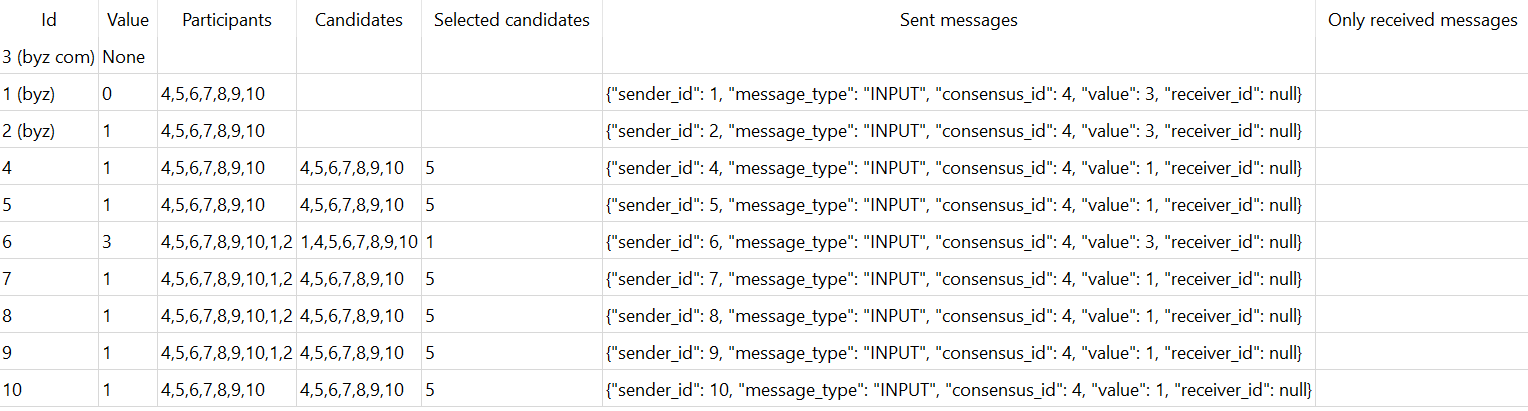
\includegraphics[width=1\textwidth]{figures/upper_part_table.png}
    \caption{The upper part of the window.\label{upper_part_table_fig}}
\end{figure}

The frontend part can show the result of the backend, the result of a given consensus round by round. It has only one mandatory argument:
\begin{itemize}
  \item input-file
\end{itemize}
\begin{figure}[hbt!]
    \centering
    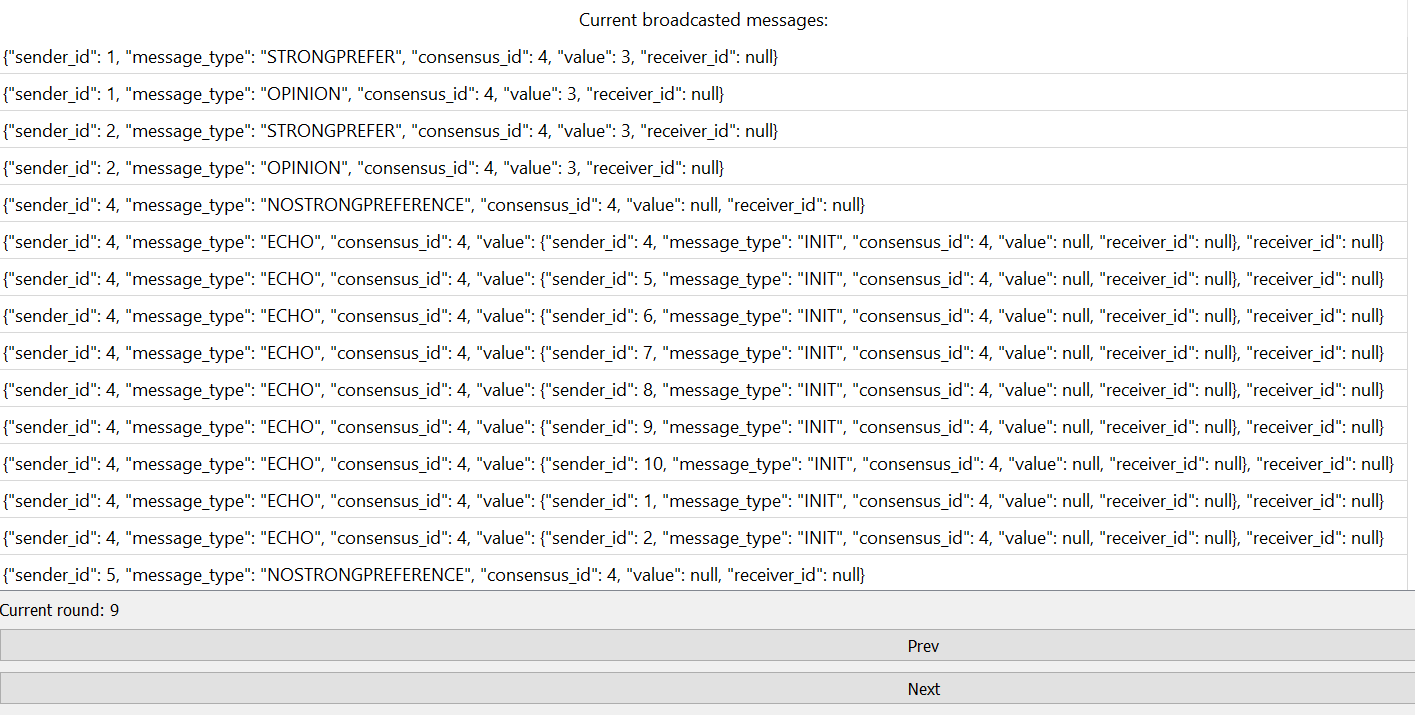
\includegraphics[width=1\textwidth]{figures/lower_part_table.png}
    \caption{The lower part of the window.\label{lower_part_table_fig}}
\end{figure}
This defines the output file path of the backend. This file contains every information about a given consensus. The frontend uses the PyQt5 visualization library to show all information from a round in a given consensus. The frontend consists of two bigger parts. The upper part of the window contains a table with information about nodes in a given round. It shows all relevant information about a node like id, current value, participants, candidates, sent messages, and only received messages. If a node is a byzantine one it is indicated in the id column. 

The lower part of the window contains all the broadcasted messages that every node gets in the given round, a text label with the current round number, and two buttons to jump between rounds.

\section{Experiments}
During the experiments all possible scenarios were studied. The repository includes these json input files for the backend and these configurations create input files for the frontend as well. The first scenario (input1.json) is the simplest - when all nodes are correct and nothing interesting can happen, because there are no byzantine nodes in the network. The second one (input2.json) has only one byzantine node which is a byzantine commander. Without other byzantine nodes, the correct nodes easily make an agreement despite the different input values. Thus after the first phase the correct nodes are terminated, because any chosen coordinator in the rotor-coordinator algorithm is correct. No other phase is necessary in this case.  The last scenario (input3.json) is the most interesting one - when there is a byzantine commander and some byzantine participants as well. In this scenario, at a given point the correct nodes have different knowledge of the network and participants. They have different participant and candidate lists as well since byzantine nodes send different messages directly to correct nodes, but this state lasts only one round because of reliable broadcast. There can be other scenarios as well, but they are as straightforward as the first one because of the consensus algorithm.

\section{Summary}
The program and experiments demonstrate Pankaj Khanchandani and Roger Wattenhofer’s  interesting and working approach of Byzantine Fault-Tolerant Consensus with Unknown Participants\cite{lamport2019byzantine}, and their algorithms solve this problem in synchronous systems with the resiliency of \(n > 3f\) as the paper claimed.

\bibliographystyle{unsrt}
\bibliography{bibliography}

\end{document}